%   Filename    : chapter_4.tex 
\chapter{Preliminary Results/System Prototype}

\section{System Architecture}
Using the tools mentioned in Section~\ref{sec:devtools}, our system can be visualized as shown in Figure \ref{fig:architecture}: 
\begin{figure}[h] % 'h' places the figure approximately here in the text
	\centering
	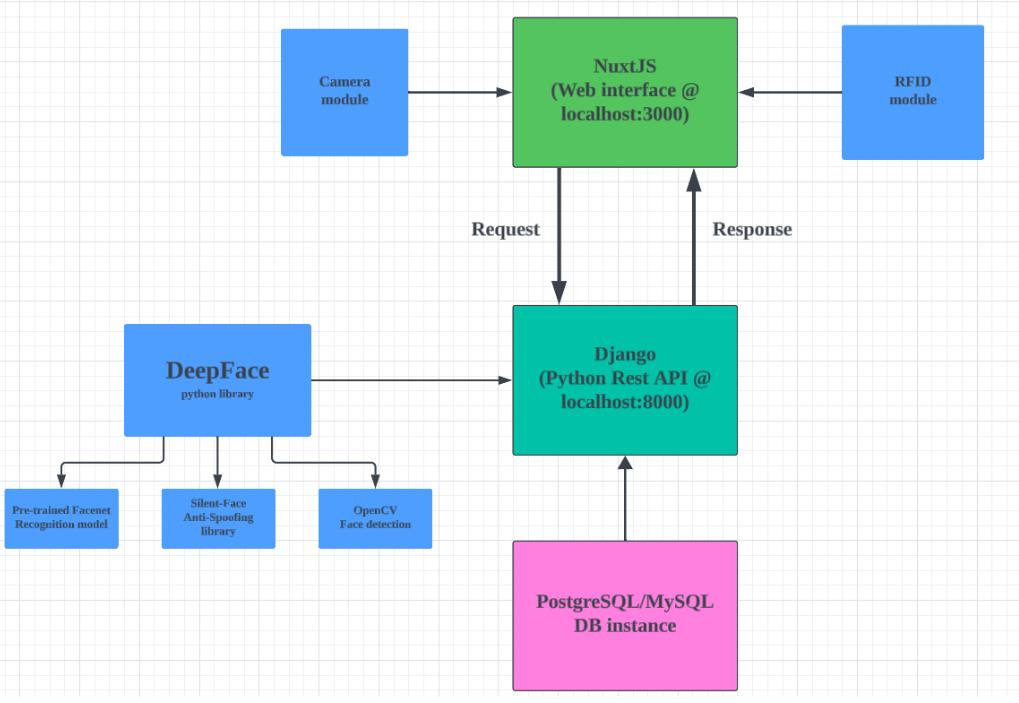
\includegraphics[width=0.8\textwidth]{figures/chapter4/architecture.png} % Adjust width as needed
	\caption{System Architecture}
	\label{fig:architecture}
\end{figure}

\section{Django Backend}
\subsection{Models}
	Django Model class maps to SQL tables. For example, a Student table will have the following columns which maps to Student Model class' attributes like in Figure \ref{fig:models}: 
	
	\begin{figure}[h] % 'h' places the figure approximately here in the text
		\centering
		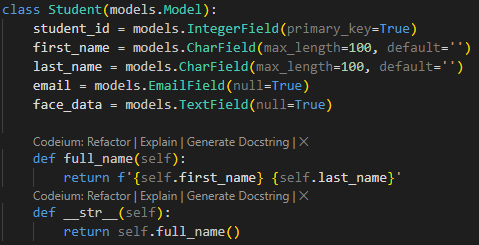
\includegraphics[width=0.8\textwidth]{figures/chapter4/models.png} % Adjust width as needed
		\caption{System Architecture}
		\label{fig:models}
	\end{figure}
	
	SQL equivalent would be:
	\begin{verbatim}
		CREATE TABLE Student (
		student_id INTEGER PRIMARY KEY,
		first_name VARCHAR(100) NOT NULL DEFAULT '',
		last_name VARCHAR(100) NOT NULL DEFAULT '',
		email VARCHAR(254),
		face_data TEXT,
		CONSTRAINT unique_email UNIQUE (email)
		);
	\end{verbatim}
	
